\documentclass{standalone}

\usepackage{tikz}
\usetikzlibrary{calc, intersections}


\begin{document}
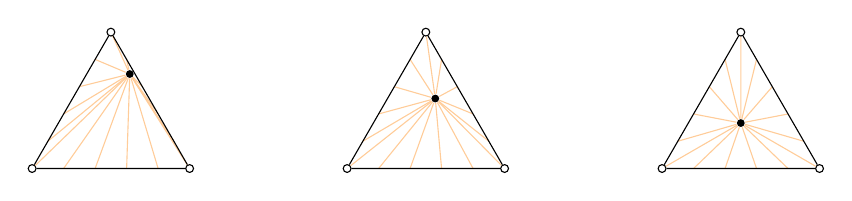
\begin{tikzpicture}[scale=2]
  \pgfmathsetmacro{\y}{sqrt(3)/2}
  \pgfmathsetmacro{\xl}{1/2}

  \def\drawss{
    % Name the vertices of the simplex
    % a
    % / \
    % c - b
    % \ /
    % d
    %
    \node[circle, draw=black, fill=white, inner sep=1pt] (a) at (0,\y) {};
    \node[circle, draw=black, fill=white, inner sep=1pt] (b) at (\xl,0) {};
    \node[circle, draw=black, fill=white, inner sep=1pt] (c) at (-\xl,0) {};
    \coordinate (mab) at ($.5*(a) + .5*(b)$);
    \coordinate (mac) at ($.5*(a) + .5*(c)$);
    \coordinate (mbc) at (0,0);

    \foreach \rat in {1,2,...,4}{
      \pgfmathsetmacro{\ratfrac}{\rat/5}
      \pgfmathsetmacro{\compratf}{1 - \ratfrac}

      \coordinate (ab\rat) at ($\ratfrac*(a) + \compratf*(b)$);
      \coordinate (ac\rat) at ($\ratfrac*(a) + \compratf*(c)$);
      \coordinate (bc\rat) at ($\ratfrac*(b) + \compratf*(c)$);
      \draw[orange!40!white] (ab\rat) -- (dpoint) (ac\rat) --
      (dpoint) (bc\rat) -- (dpoint);
    }

    % Draw the lines from the vertices to the moving point
    \draw[orange!40!white] (a) -- (dpoint) (b) -- (dpoint) (c) -- (dpoint);
    \coordinate (baanc) at (-0.26689486636167326, -0.40374993496671496);
    \coordinate (bbanc) at (-0.0631834845621597, -0.7565883983235342);
    \pgfmathsetmacro{\bat}{0.6898382210948677}
    \pgfmathsetmacro{\bbt}{0.3449191105474339}
    \pgfmathsetmacro{\batc}{1-\bat}
    \pgfmathsetmacro{\bbtc}{1-\bbt}

    % \node[circle, draw=black, fill=white, inner sep=1pt] (b1) at ($\bat*(dpoint) + \batc*(baanc)$) {};

    % \coordinate (mbc) at (0,0);

    % \draw[dotted] (a) -- (b1) (b) -- (b1) (c) -- (b1) (mab) -- (b1)
    % (mac) -- (b1) (mbc) -- (b1);


    % Draw boundary of simplex
    \draw (a) -- (b) -- (c) -- (a);

  }

  % Start point and endpoint
  \coordinate (v) at (0.12, 0.6);
  \coordinate (u) at (0.0, 0.28867513459481287);


  \coordinate (spoint) at (v);
  \coordinate (epoint) at (u);

  \begin{scope}[xshift=-2cm]
    \coordinate (sspoint) at ($(spoint) + (-2.,0.)$);
    \node[circle, fill=black, inner sep=1pt] (dpoint) at ($(sspoint) +
    (0.,0.)$) {};
    \drawss
  \end{scope}

  \begin{scope}[xshift=0cm]
    \coordinate (sspoint) at (spoint);
    \node[circle, fill=black, inner sep=1pt] (dpoint) at
    ($.5*(spoint) + .5*(epoint)$) {};
    \drawss
  \end{scope}

  \begin{scope}[xshift=2cm]
    \coordinate (sspoint) at ($(spoint) + (2.,0.)$);
    \coordinate (epoint) at ($(epoint) + (2., 0)$);
    \node[circle, fill=black, inner sep=1pt] (dpoint) at
    (epoint) {};
    \drawss
  \end{scope}
\end{tikzpicture}
\end{document}
